% Graphs (1 week)

Graphs are an important abstract data structure that underlie graph theory in theoretical computer science. They are important for chemistry because they can be a suitable way of representing molecules.

\begin{itemize}
    \item \textbf{Node/ Vertex:} Object with name and data (in context of molecules: the atoms)
    \item \textbf{Edge:} Connection between two vertices (in context of molecules: the bond)
    \begin{itemize}
        \item Can be weighted (in context of molecules: single bond and double bond)
        \item Can be directed 
    \end{itemize}
    \item \textbf{Graph:} Collection of nodes and edges
    \begin{center}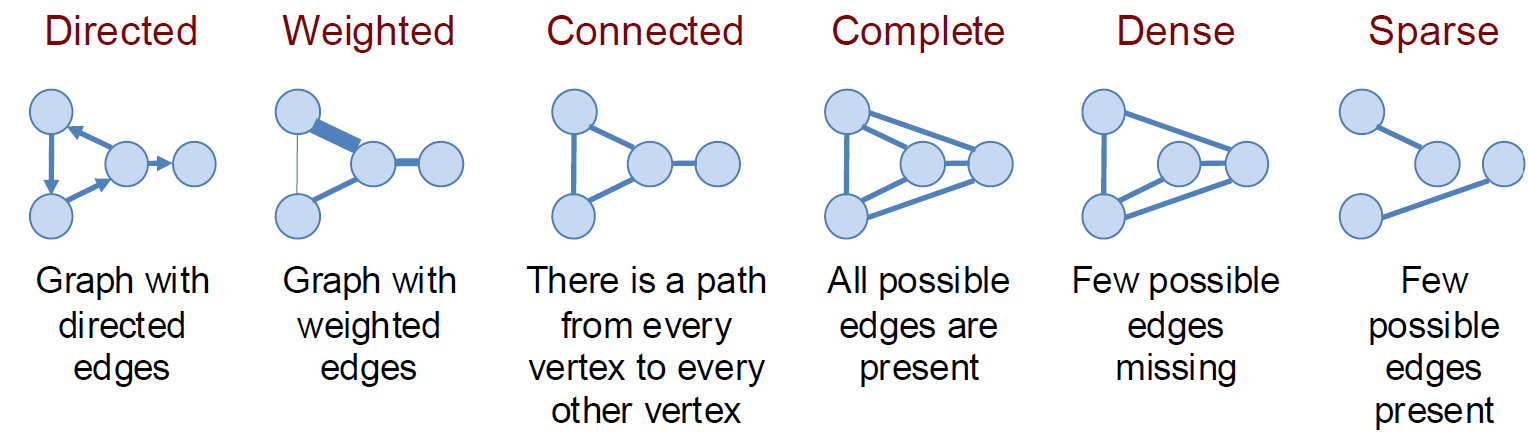
\includegraphics[width=0.85\textwidth]{img/graphs/DifferentGraphs.png}\end{center}
    \item \textbf{Valence of degree of vertex:} Number of edges a vertex lies on (in context of molecules: valence)
    \item \textbf{Adjacent vertices:} Vertices connected by an edge (in context of molecules: neibouring atoms)
    \item \textbf{Path:} List of distinct vertices in which successive vertices are connected by edges
    \begin{itemize}
        \item Simple Path: path with no vertex occurring twice
        \item Cycle Path: simple path of which first and last vertex are the same
    \end{itemize}
    \begin{center}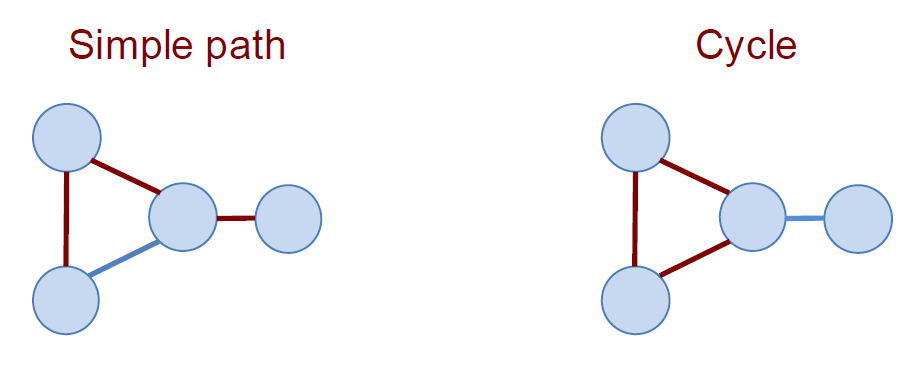
\includegraphics[width=0.45\textwidth]{img/graphs/PathGraphs.png}\end{center}
    \item \textbf{Trees:} (in graph theory)
    \begin{itemize}
        \item \textbf{Tree:} non-empty, acyclic collection of nodes and edges (graph) in which any 2 nodes are connecteds by exactly 1 path.  
        \item \textbf{Ordered Tree:} tree with order in the children nodes
        \item \textbf{Binary Tree:} ordered tree in which each non-terminal node has exactly two children
        \item \textbf{Binary Search Tree:} ordered binary tree with left-to-right order
        \item \textbf{Heap:} ordered binary tree with top-to-bottom order
    \end{itemize}
    \begin{center}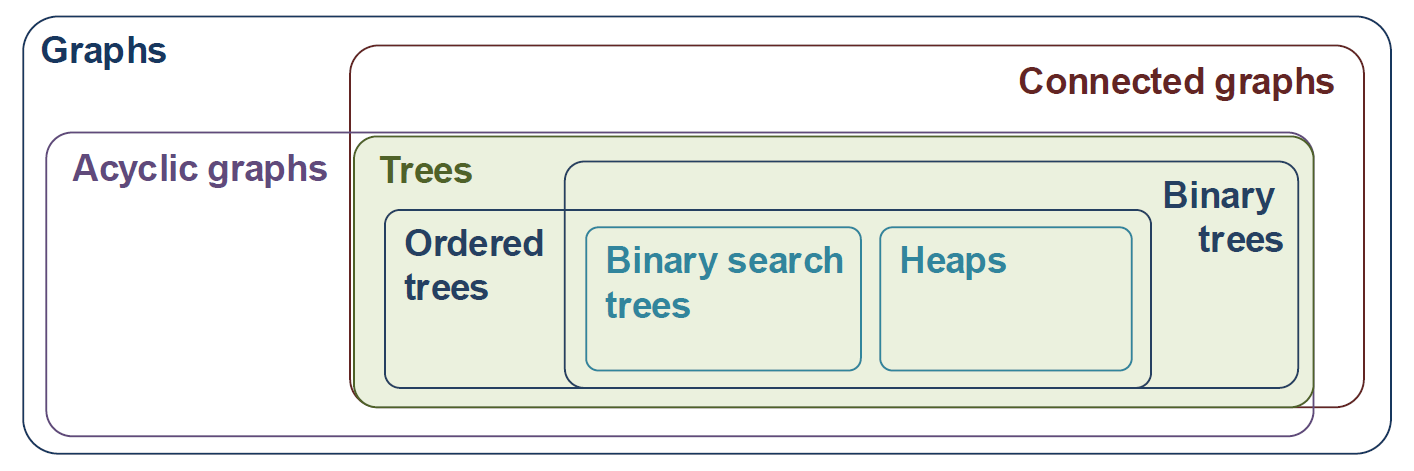
\includegraphics[width=0.75\textwidth]{img/graphs/GraphsTrees.png}\end{center}
\end{itemize}

\subsection{Representations of graphs}

A graph $G(V,E)$ with vertices $V$ and edges $E$ can be represented as a adjacency matrix (good for dense graphs) or an adjacency list (good for sparse graphs). 

\begin{center}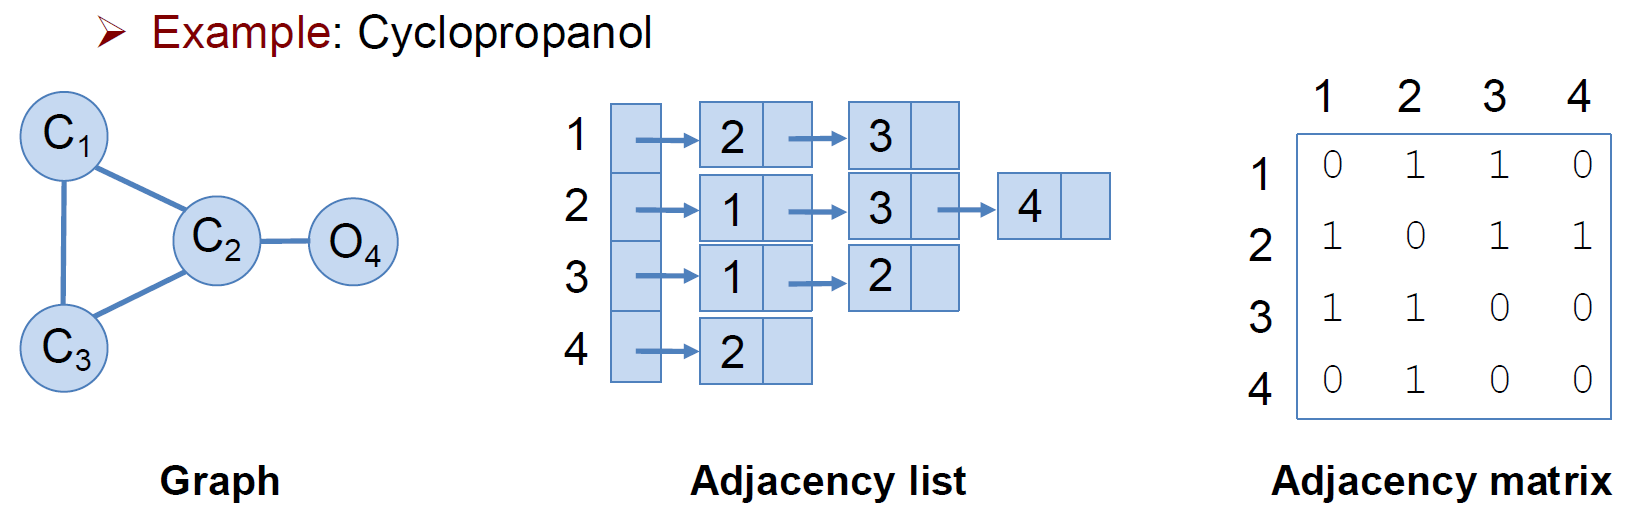
\includegraphics[width=0.85\textwidth]{img/graphs/MatrixVsList.png}\end{center}

\begin{table}[H]
    \centering
    \begin{tabular}{p{30mm} | p{50mm} | p{50mm}}
        \toprule
        \textbf{Function} & \textbf{Adjacency list} & \textbf{Adjacency matrix} \\
        \midrule
        \lstinline|size()| & Easy, size of a vector & Easy, size of a vector \\
        \midrule
        \lstinline|isConnected()| & Difficult, search in linked list & Easy, direct access \\
        \midrule
        \lstinline|getNeighbours()| & Easy, copy of linked list & Difficult, search in row \\
        \midrule
        \lstinline|addEdge()| & Easy, append linked list & Easy, set matrix element to 1 \\
        \bottomrule
    \end{tabular}
\end{table}

\subsubsection{Adjacency list}

When implemented as a linked list for a graph, the central data storage is via a vector of linked lists, whereby a linked list exists for each vertex with all connected vertices. The biggest advantage is that the memory is used optimally with $\Theta(V+E)$. However, the biggest disadvantage is that there is no really fast way to check whether an edge exists.

%\lstinputlisting[language=C++]{src/graphs/graph_list.cpp}

\subsubsection{Adjacecy matrix}

When implemented as a matrix for a graph, the central data storage is a $V\times V$ matrix $A$ (vector of a vector), whose entries $a_{ij}$ represent the edge weight between vertex $i$ and $j$. The biggest advantage of this form is the simple implementation and verification of edges. However, the matrix requires a relatively large amount of memory, at $\Theta(V^2)$.

%\lstinputlisting[language=C++]{src/graphs/graph_matrix.cpp}

\subsection{Searching a graph}

When searching for a vertex in a graph, two different algorithms can be used: the first depth-first, the second breadth-first.

\subsubsection{Breadth-first (BF) search}

The breadth-first algorithm starts with a specific source vertex $s$, from which all vertices that can be reached from $s$ are discovered. This creates a breadth-first tree with the root $s$ and all reachable vertices.  During the algorithm, the shortest path (distance) from $s$ to $v$ is also determined for each vertex $v$. The vertices have three possible states:

\begin{itemize}
    \item \textbf{white:} undiscovered
    \item \textbf{gray:} discovered but with undiscovered neighbours
    \item \textbf{black:} discovered and all neighbours are discovered as well
\end{itemize}

All gray vertices are in a queue so that they can be processed one after the other. The running time of the algorithm is $\Theta(V+E)$.

Procedure:
\begin{enumerate}
    \item First, only the given root $s$ is gray.
    \item All neighboring vertices of $s$ become gray, their distance is 1 and $s$ becomes black.
    \item All neighbors of the gray vertices become gray, their distance is 2 and the former gray vertices become black. The gray vertices in the queue are processed one after the other.
\end{enumerate}

\begin{center}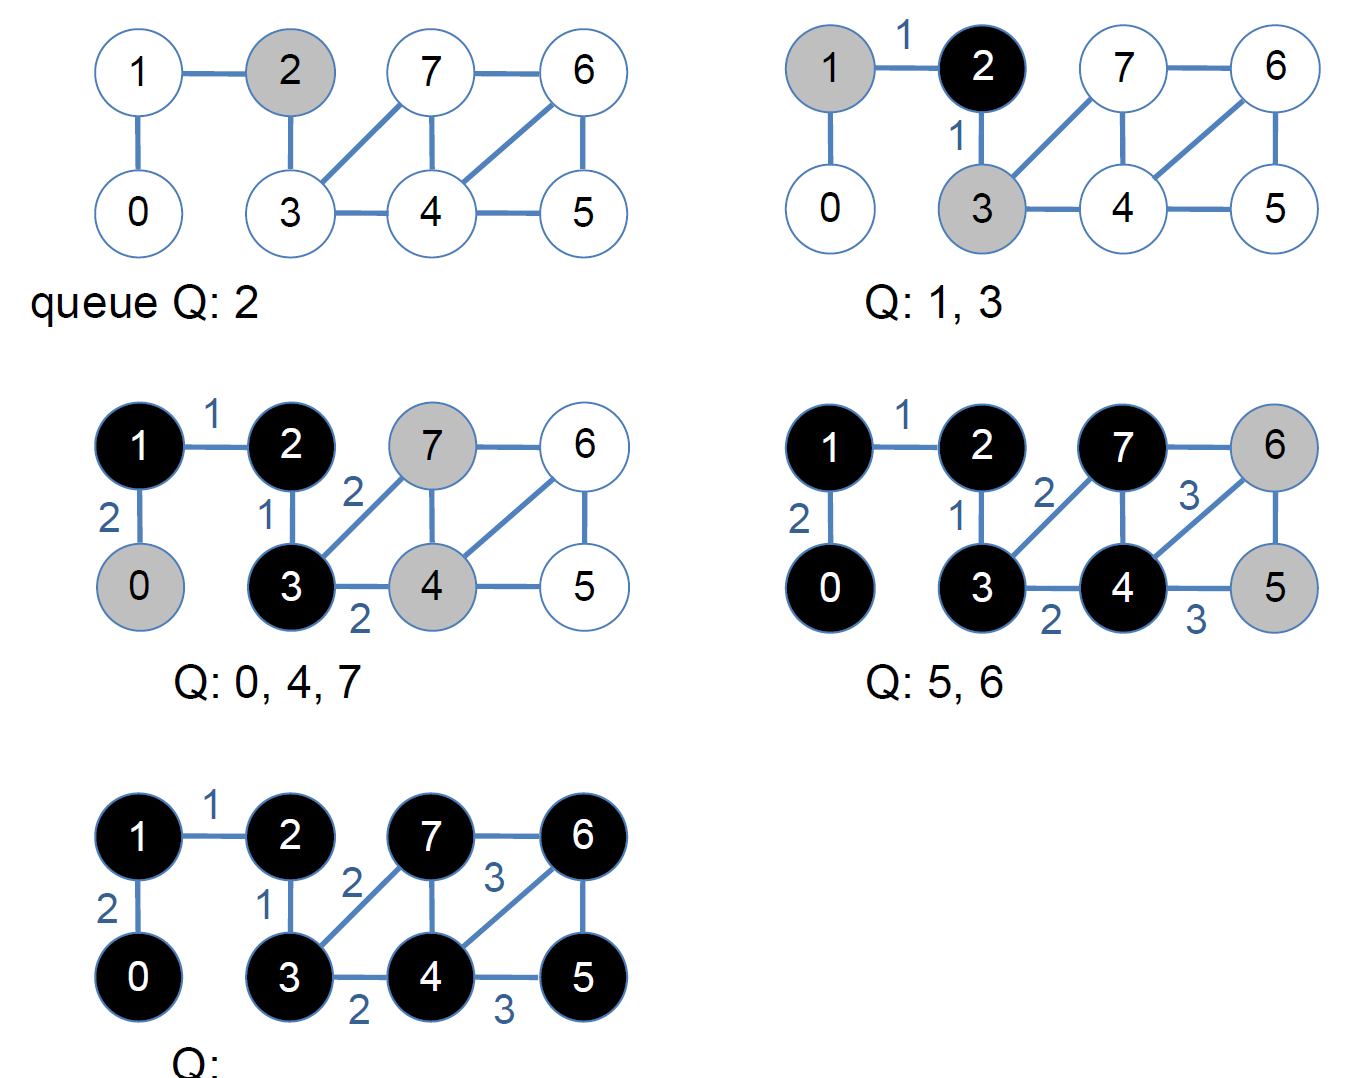
\includegraphics[width=0.65\textwidth]{img/graphs/BfSearch.png}\end{center}

% finished code, but without outpur of the searching
%\lstinputlisting[language=C++]{src/graphs/bf_search.cpp}

\subsubsection{Depth-first (DF) search}

If possible, the depth-first algorithm always searches deeper in the tree first and not as broadly as possible as with the BF algorithm. This creates a depth-first forest. Here, too, you start with a source vertex $s$ and discover all vertices that can be reached via $s$, but the three classifications of the vertices are slightly different:

\begin{itemize}
    \item \textbf{white:} undiscovered
    \item \textbf{gray:} first discovered (time $d$)
    \item \textbf{black:} all neighbours are discovered (time $f$)
\end{itemize}

The running time of the algorithm is $\Theta(V+E)$. If vertices remain after the algorithm that cannot be reached from the source $s$, the algorithm is continued via a new source $s$.

Procedure:
\begin{enumerate}
    \item First, only the given root $s$ is gray. (0)
    \item Then the neighbor of $s$ becomes gray with the smallest value. (1)
    \item Then the neighbor of (1) with the smallest value is grayed out again. (2) This continues until a vertex is found that has no neighbors. (3)
    \item Now the backtracking begins until a vertex is found that still has unexplored neighbors. This then turn gray and the procedure continues.
\end{enumerate}

\begin{center}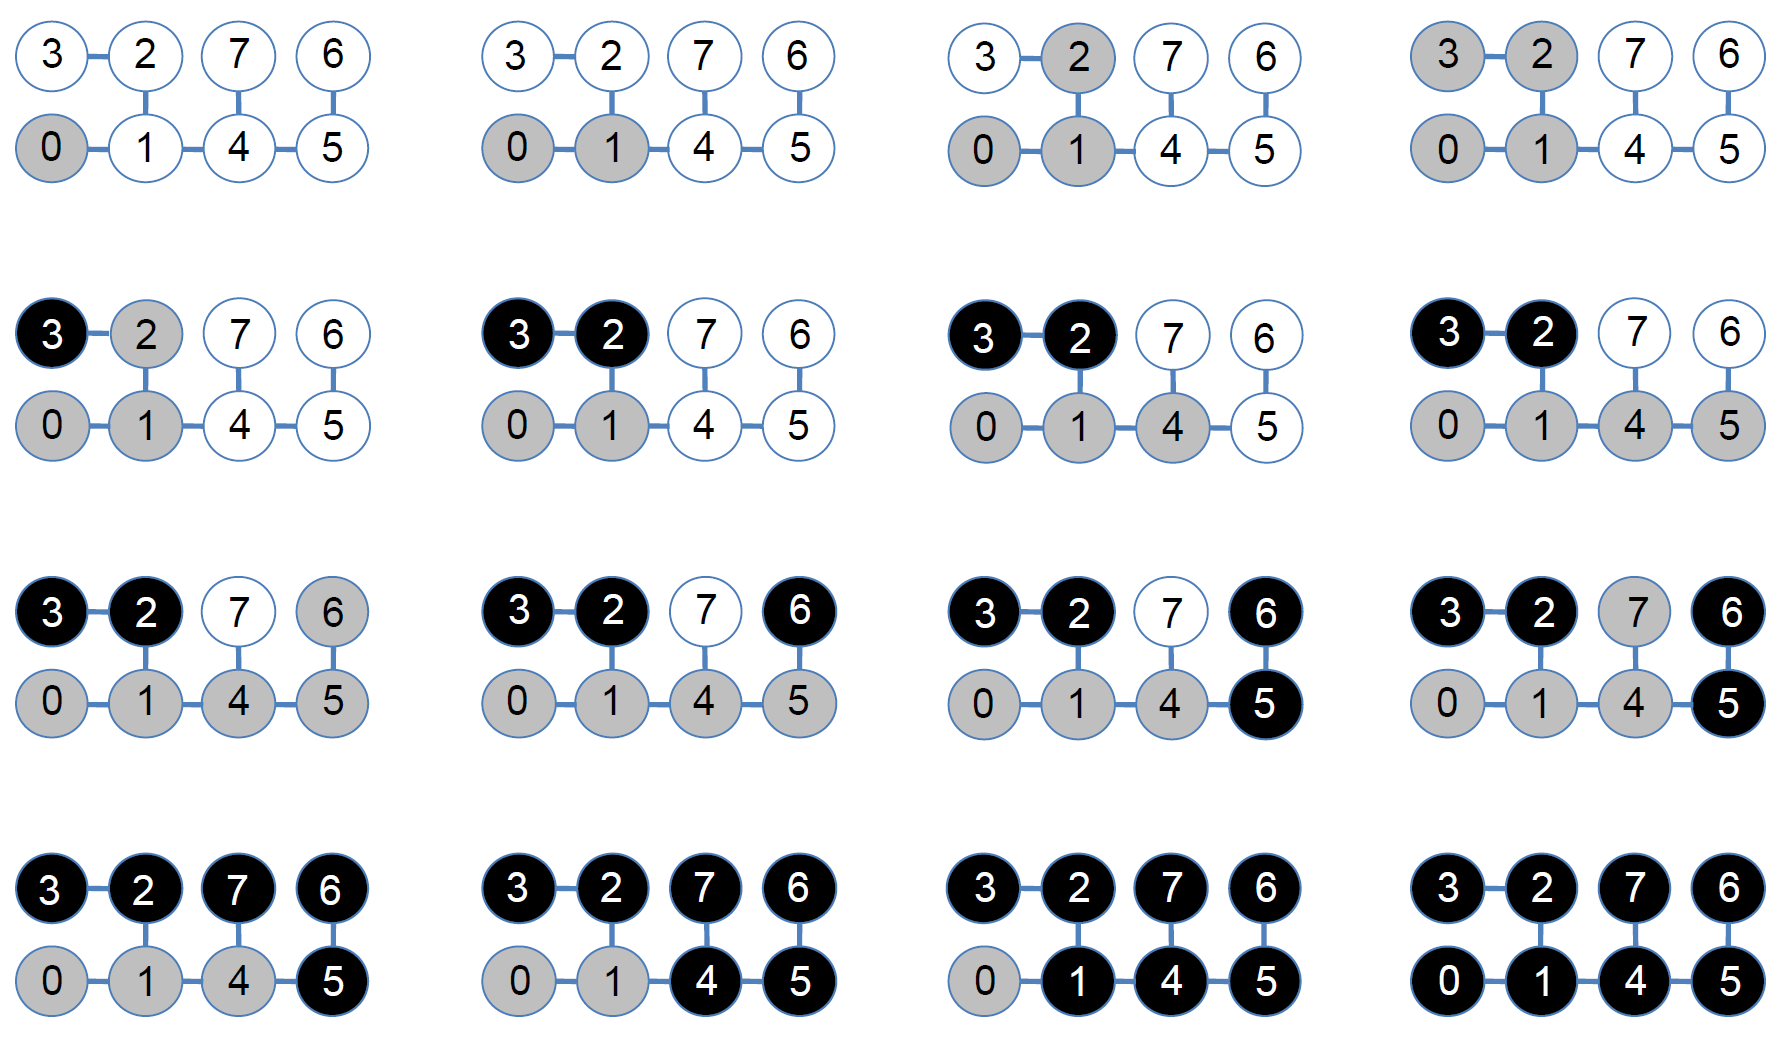
\includegraphics[width=0.85\textwidth]{img/graphs/DfSearch.png}\end{center}

% finished code, but without outpur of the searching
%\lstinputlisting[language=C++]{src/graphs/df_search.cpp}

\subsection{Minimum spanning trees}

The \emph{minimum spanning trees problem} is to turn a graph into a tree such that all vertices are connected and the sum of the edge weights is minimal. An important property of this tree is that if the vertices of the graph are arbitrarily divided into two sets, the minimum spanning tree always contains the shortest path between two vertices from both sets. In principle, two algorithms can be applied to the problem, namely \emph{Kruskal's algorithm} (good for sparse graphs) and \emph{Prim's algorithm} (good for dense graphs), which both run in $\Theta(E\lg V)$ time for a graph $G(V,E)$ with vertices $V$ and edges $E$.

\begin{center}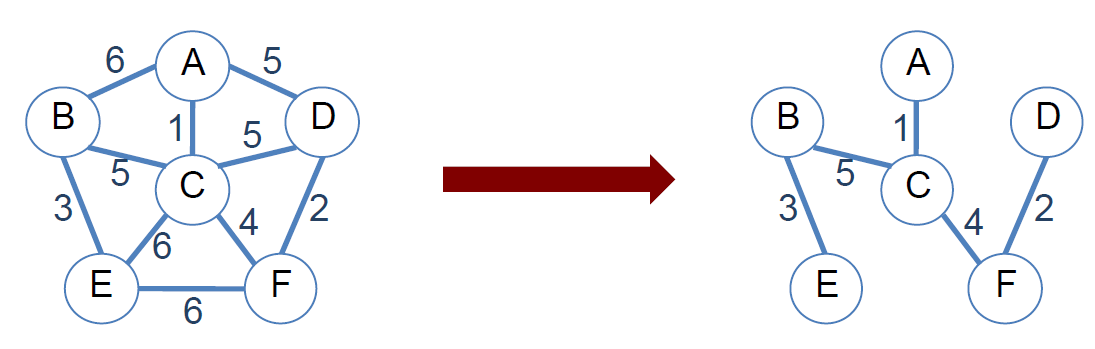
\includegraphics[width=0.70\textwidth]{img/graphs/MinimumSpanningTree.png}\end{center}

\subsubsection{Kruskal's algorithm}

In \emph{Kruskal's algorithm}, the minimum spanning tree is constructed by joining a set of unconnected vertices together. The tree is therefore built from the root and no edges are deleted, which is why it is particularly suitable for sparse graphs. It is a greedy algorithm with $\Theta(E\lg V)$ that follows the following procedure:

\begin{enumerate}
    \item Put the edge with the lowest weight in a tree of the forest
    \item Put the edge into the forest with the next higher weight (algorithm follows ascending weights), provided that adding it does not create a cycle. If it does, skip that edge.
    \item Stop after $V-1$ edges have been considered (ensures that all vertices are connected to each other). 
\end{enumerate}

\begin{center}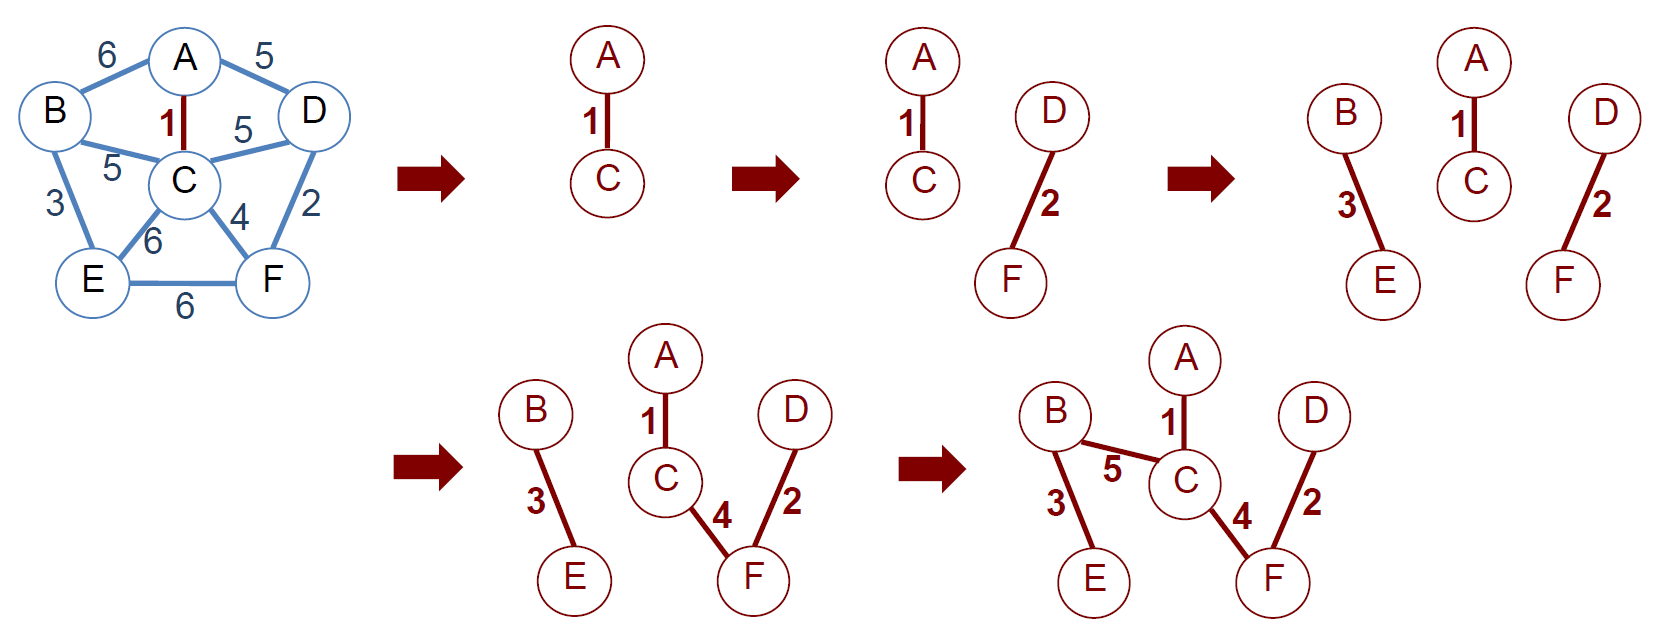
\includegraphics[width=0.85\textwidth]{img/graphs/KruskalGraph.png}\end{center}

%\lstinputlisting[language=C++]{src/graphs/kruskal.cpp}

\subsubsection{Prim's algorithm}

\emph{Prim's algorithm} is a greedy algorithm with $\Theta(E\lg V)$ that follow the follwoing procedure:

\begin{enumerate}
    \item Put one random vertex on the tree (e.g. A)
    \item Find the edge with the lowest weight that connects A to a vertex, that is not in the tree yet. (C)
    \item Find from C the edge with the lowest weight that connects C to a vertex, that is not in the tree yet, but without building a cycle. (F)
    \item Continue finding edges with the lowest weight from the last vertex without building a cycle. If there is no edge to a vertex, without building a cycle, go back until you have a vertex with new neighbours.
    \item Stop if tree contains $V$ vertices or if no more edges can be found.
\end{enumerate}

\begin{center}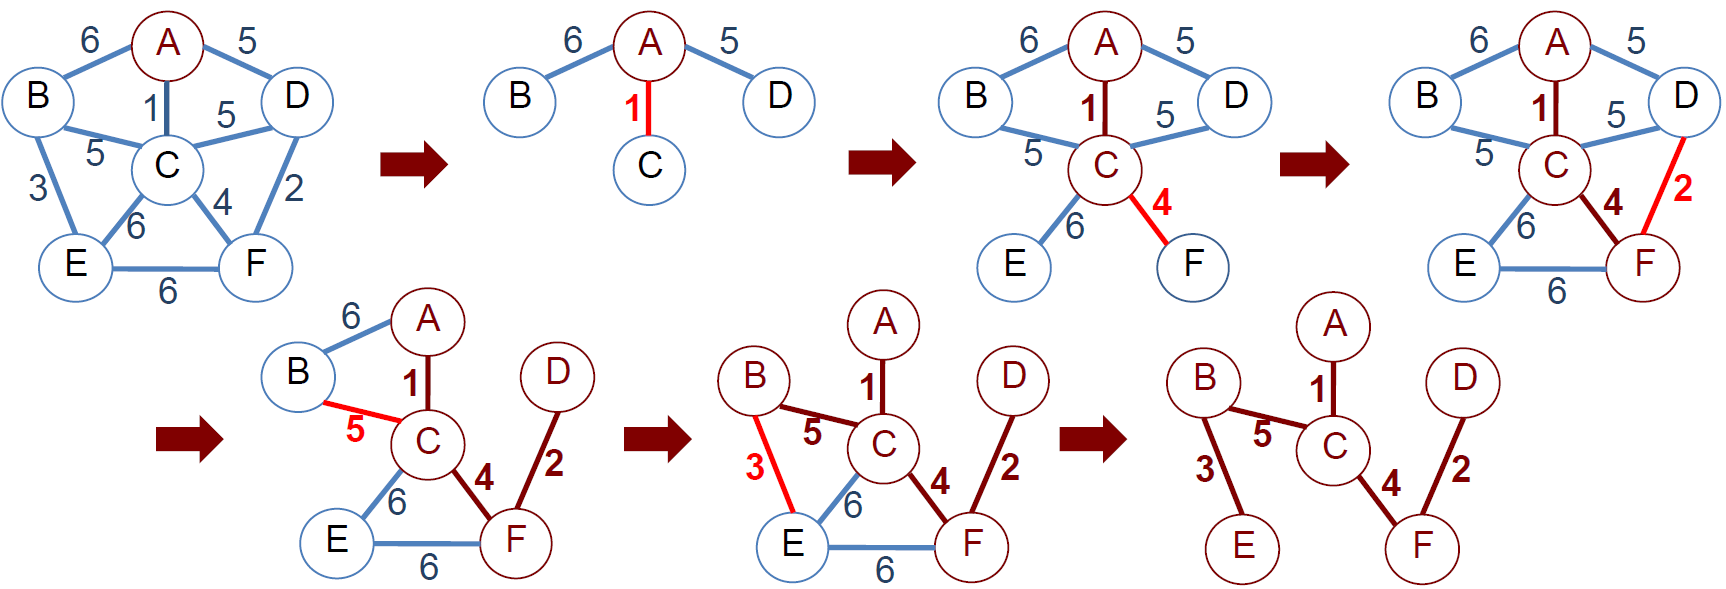
\includegraphics[width=0.85\textwidth]{img/graphs/PrimGraph.png}\end{center}

%\lstinputlisting[language=C++]{src/graphs/prim.cpp}

\subsection{Single-source shortest paths}

The \emph{Single-source shortest paths} problem is to determine the length $d_i$ of the shortest path from the source vertex $v_0$ (single source) to every other vertex $v_i$. For that we use an directed and weighted graph (only positive weights and directed edges) and the length $d_i$ of the path is the sum of the weights along its edges. One can use in principle two algorithms for that:

\begin{itemize}
    \item \textbf{Brute-force:} Try all combinations of edges with $\Theta((V-1)!)$
    \item \textbf{Dijkstra's algorithm} Greedy algorithm with $\Theta(V^2)$
\end{itemize}

\subsubsection{Dijkstra's algorithm}

Dijkkstra's algorithm is a greedy algorithm that can find the weight or distance $d_i$ of the shortest path from a given source vertex 
$v_0$ to each other vertex $v_i$ of the graph. It runs in a running time of $\Theta(V^2)$, which can be improved to $\Theta((V+E)\lg V)$ for a sparse graph and to $\Theta(E\lg V)$ for a sparse graph in which all vertices can be reached from the source vertex. To do this, the algorithm defines two sets of vertices:

\begin{itemize}
    \item Vertices that were already considered: Their shortest path is known.
    \item Vertices that have not been considered yet. 
\end{itemize}

During the algorithm, a distance table, which is initially the adjacency matrix of the graph, is continuously updated. The weights of the paths from all vertices to the source vertex are stored in a vector.

\begin{enumerate}
    \item First, determine the direct distance $d_i$ from the source vertex $v_0$ to each vertex $v_i$ of the graph ($d_i=\mathrm{weight}(v_0,v_i)$) and insert the distances into the path vector.
    \item Create a vector of the size of all vertices, which is initially set to zero for all elements. If a vertex has been taken into account, the vector element for this vertex becomes one. 
    \item Make a loop over all vertices (An index k is defined which maps to the vertex currently being considered, but which is not the loop index. At the beginning: $k=v_0$):
    \begin{enumerate}
        \item Identify the vertex that is at the smallest distance from the source vertex $v_0$ and was not considered yet (the distances of the path vector are used). This vertex has now been taken into account, is now the current vertex and is set to one in the consideration vector.
        \item Go over all vertices that have not yet been considered and check whether the shortest path to the current vertex $v_k$ plus the distance to the new vertex is smaller than the distance stored in the path vector. If yes. update the path vector.
    \end{enumerate}
\end{enumerate}

\begin{center}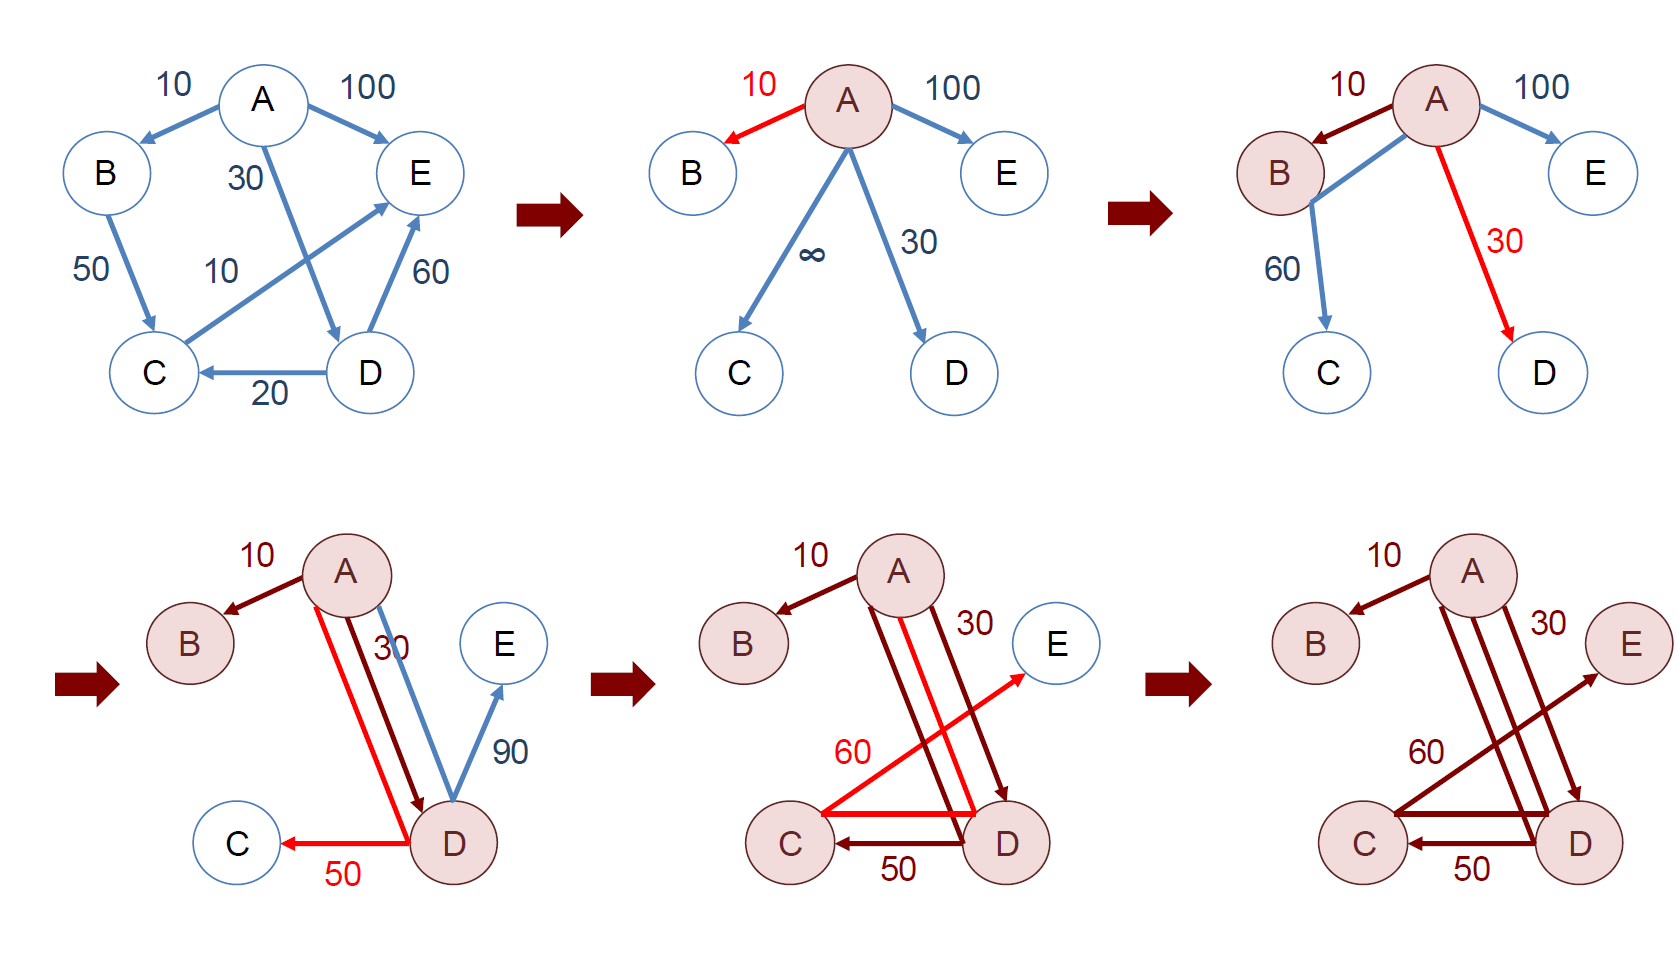
\includegraphics[width=0.85\textwidth]{img/graphs/DijkstraGraph.png}\end{center}

\begin{center}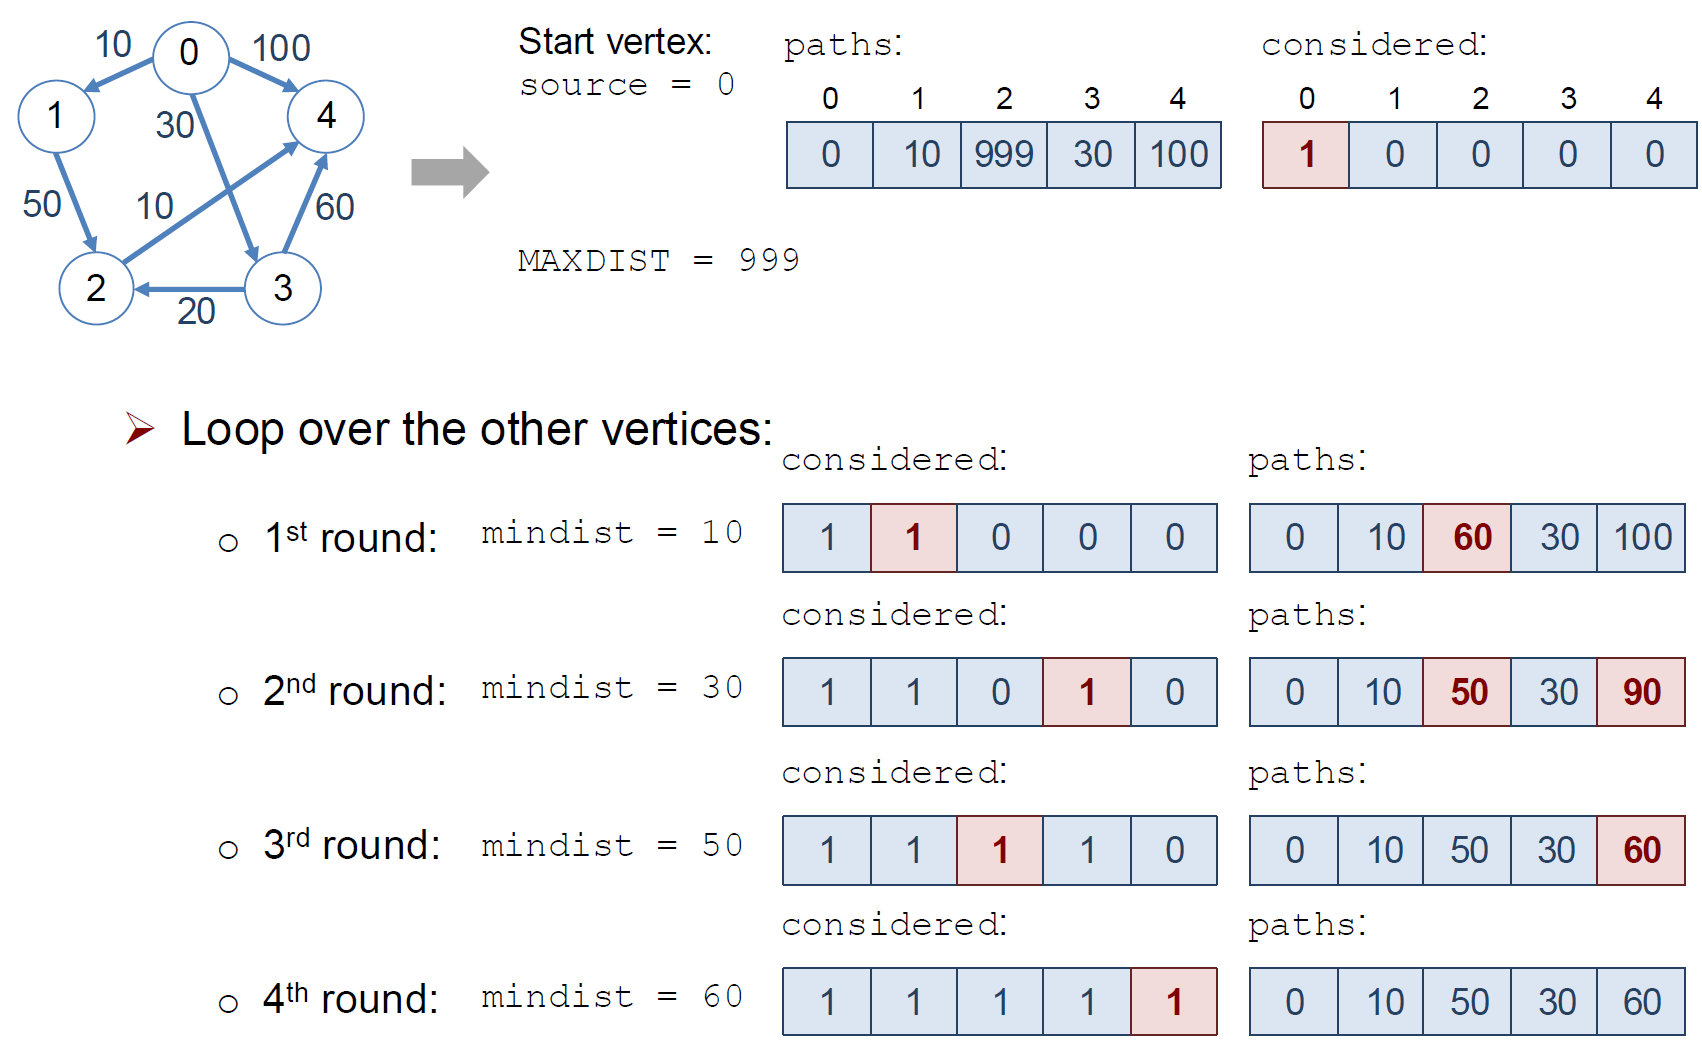
\includegraphics[width=0.85\textwidth]{img/graphs/DijkstraVectorGraph.png}\end{center}

%algorithmus ist fertig
%\lstinputlisting[language=C++]{src/graphs/dijkstra.cpp}

\subsection{All-pair shortest paths}

The \emph{All-pair shortest paths} problem is to do the single-source shortest paths problem on every vertex of a graph so that you get the length $d_{ij}$ of the shortest path between every two vertices of the graph. Here negative weights of the edges are also possible. For this problem you can choose between two algorithms.

\begin{itemize}
    \item \textbf{Dijkstra's algorithm starting at each vertex}
    \begin{itemize}
        \item Only if weights are all positive
        \item Running time: $\Theta(V^3)$ (With improvements: $\Theta(V(V+E)\lg V)$ or $\Theta(VE\lg V)$)
        \item Good for sparse graphs
    \end{itemize}
    \item \textbf{Floyd-Warshall algorithm}
    \begin{itemize}
        \item Running time: $\Theta(V^3)$
        \item Good for dense graphs
    \end{itemize}
\end{itemize}

\subsubsection{Floyd-Warshall algorithm}

The Floyed-Warshall algorithm is a \emph{dynamic programming} algorithm to determine the shortest path between each vertex of a graph and, unlike the Dijkstra's algorithm, can also handle negative edge weights. The running time is $\Theta(V^3)$, but the inner loop is very simple. The idea of the algorithm is to compare all possible paths in the graph and to build an increasingly better distance matrix to determine the shortest paths. To do this, it checks for each vertex whether it is better to take the direct route from $v_i$ to $v_j$ or to include the vertex $v_k$ as an intermediate step.

\begin{enumerate}
    \item Loop over all vertices $k$
    \item Check for each pair of vertices $v_i$ and $v_j$ whether the distance $d_{ij}$ can be made shorter via vertex $v_k$
    \begin{itemize}
        \item \lstinline|shortestPath(i,j,k)| returns the shortest possible path from $v_i$ to $v_j$ using only vertices from the set $\{1,2,\cdots,k\}$
    \end{itemize}
\end{enumerate}

\begin{center}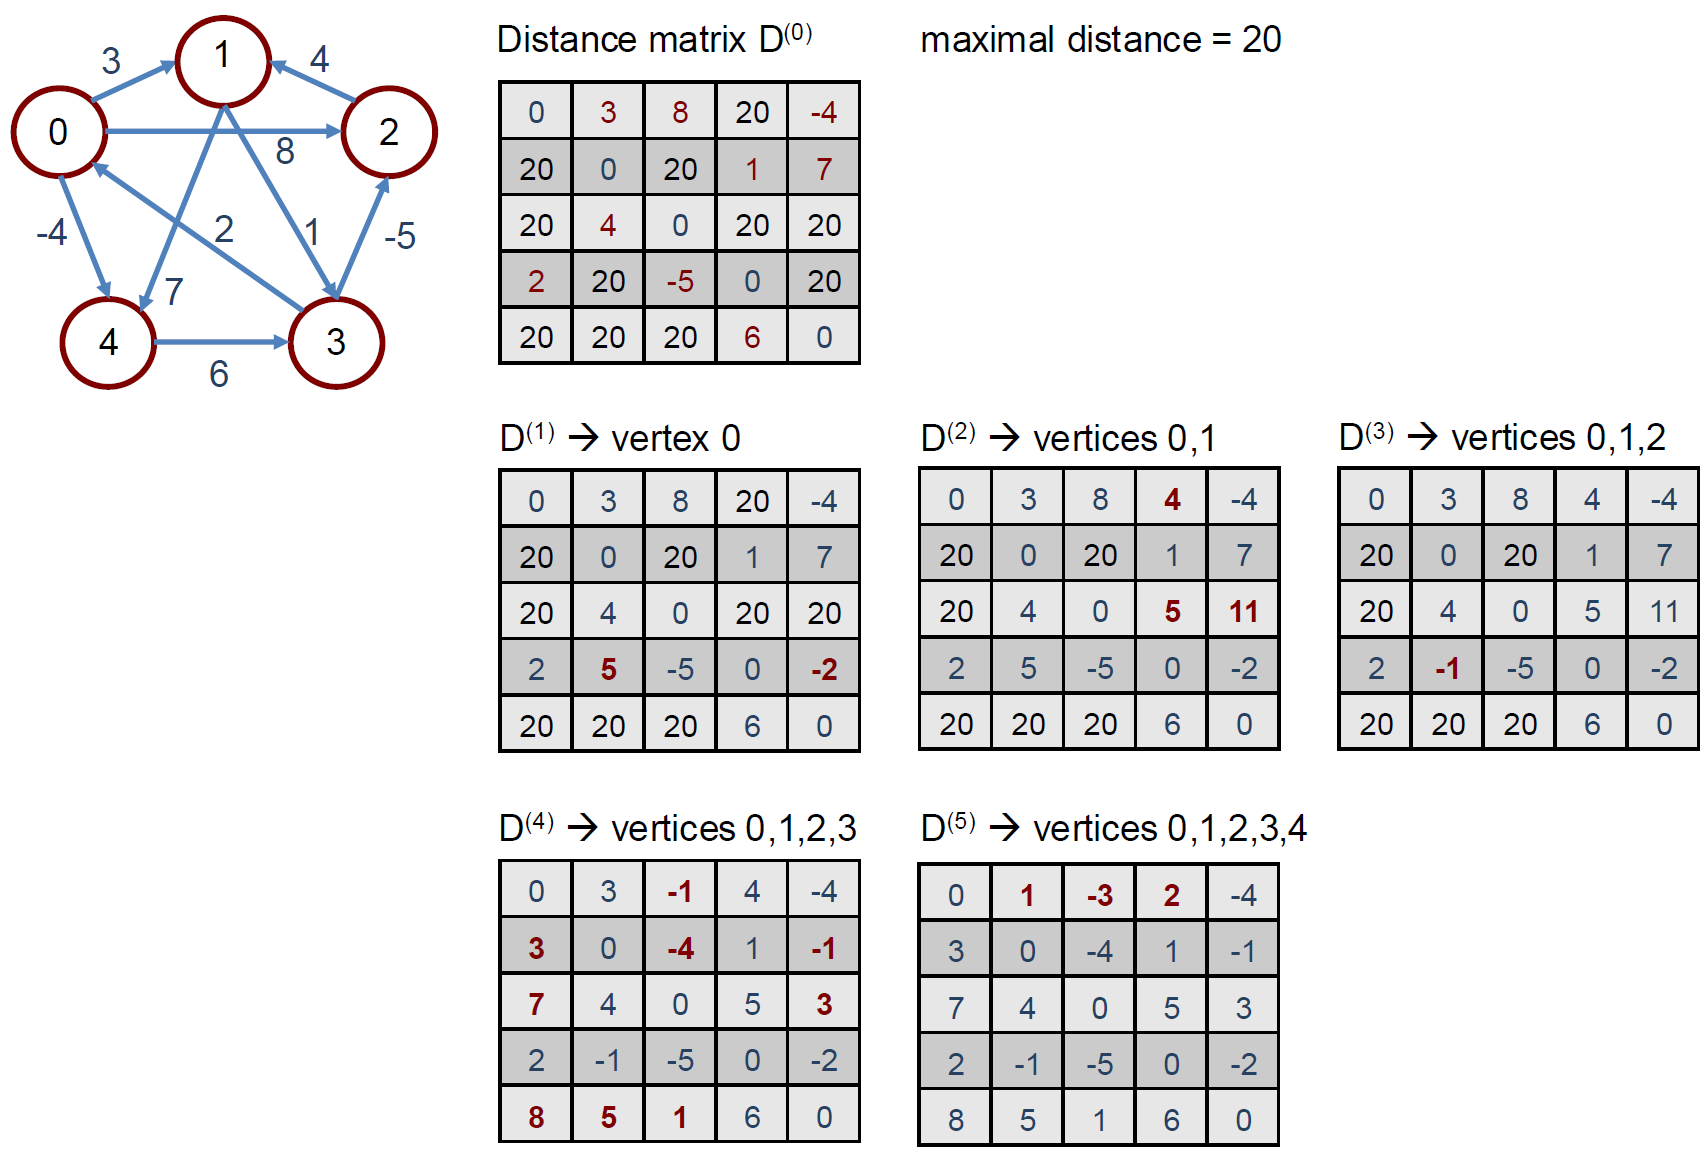
\includegraphics[width=0.85\textwidth]{img/graphs/FloydWarshallGraph.png}\end{center}

%algorithmus ist fertig
%\lstinputlisting[language=C++]{src/graphs/floyed_warshall.cpp}